%!TEX root = paper.tex
%%%%%%%%%%%%%%%%%%%%%%%%%%%%%%%%%%%%%%%%%%%%%%%%%%%%%%%%%%%%%%%%%%%%%%%%%%%%%%%%
\section{Examining Individual Lag Components}
\label{sec:lagmodel}

\begin{figure*}[t]
	\centering
	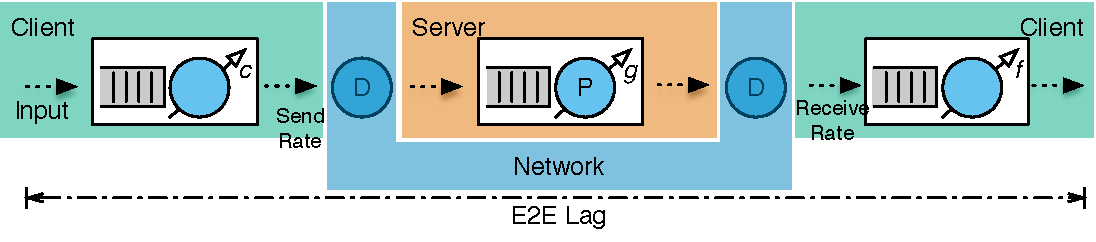
\includegraphics[width=1.0\textwidth]{images/e2e-lag-model.pdf}
	\caption{End-to-end lag model used as basis for this investigation. Several processes are assumed to be clocked, denoted by the diagonal arrows.}
\label{fig:e2e-lag-model}
\end{figure*}

In any video game a multitude of cogs is working in unison to transform a player's inputs into meaningful actions inside the game world. A simplified depiction of the processes a player action must go through before finally being to able to be displayed in a multiplayer game with an authoritative server is given in Fig.~\ref{fig:e2e-lag-model}. 

Besides additional lag incurred through the input and output devices' hardware (i.e. in this case mouse, keyboard, and monitor) --- which can on their own still be significant\footnote{See, e.g. the investigation of keyboard latency at \url{https://danluu.com/keyboard-latency/}, in some cases exceeding \SI{50}{\milli\second}.}. The components (and the corresponding terminology) investigated here are outlined in \cite{Metzger+2016}, and are 
%
\begin{itemize}
	\item the generation of the input events by the player,
	\item the command message send process (from the client to the server),
	\item the network round-trip time,
	\item the server's game state update rate (i.e. the so-called ``tick rate''),
	\item the server's update send rate (server to clients),
	\item the client's frame rate (and additionally other lag-inducing factors at the client).
\end{itemize}
%
It should be noted, that there are usually certain lag compensation techniques \cite{bernier2001latency} in place that can conceal parts of the lag from the player by speculatively displaying the player's action's results before being confirmed by the remote server. The specific measures that Overwatch takes have not yet been further examined.

For this experiment several regular matches (i.e. Overwatch's default mode with two teams of six players each) were played from the perspective of one player on one PC that can not maintain a stable frame rate of \SI{60}{\hertz} throughout the match. Packet traces of the game's incoming and outgoing encrypted UDP traffic were recorded on the same PC and are the basis for this examination. 

The code for models derived here as well as the refined lag simulation for this game is available in the public repository that hosts this paper.\footnote{\url{https://github.com/fmetzger/overwatch-lag-model}}
The following sections each examine one of individual behavioral components of the game, as shown in the overview in Fig.~\ref{fig:e2e-lag-model}.


\subsection{Command Messages}

% TODO: state the nature of this figure: it is a fringe case, no such behavior could be observed on a computer with sufficient resources (and thus stable \SI{60}{\hertz} frame rate)
\begin{figure}[t]
	\centering
	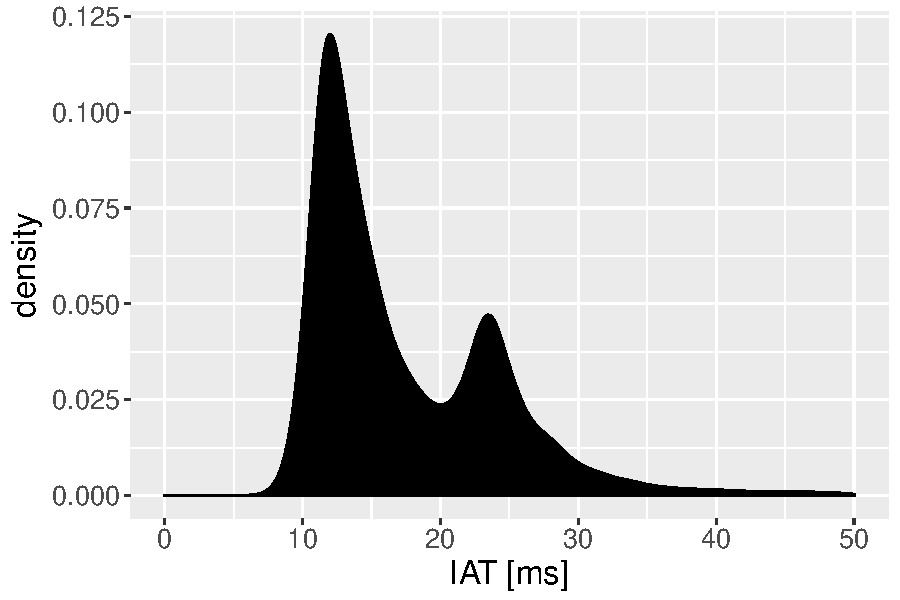
\includegraphics[width=1.0\columnwidth]{images/command-density.pdf}
	\caption{Continuous density plot of the command messages the client sends, showing a bimodal behavior instead of the expected single mode at \SI{16.7}{\milli\second}.}
\label{fig:command-density}
\end{figure}

The command messages are the messages the game clients sends to the server, containing all the player's inputs during that cycle. The developers of \textsc{Overwatch} advertise a tick rate (i.e. the frequency the server updates its game state) of \SI{60}{\hertz} (or an \gls{IAT} of about \SI{16.7}{\milli\second}. Therefore, one would assume that the game's transmission behavior targets the same values to incorporate all player decisions (i.e. inputs) in each update cycle and notify them of the resulting game state.

However, when looking at the density of the command message \glspl{IAT} in Fig.~\ref{fig:command-density}, actually two modes are revealed, one at around \SI{24}{\milli\second} (or a send rate of \SI{42}{\hertz}) and the other one at \SI{12}{\milli\second} (\SI{83}{\hertz}). Even though the overall mean \gls{IAT} is \SI{17.9}{\milli\second} and thus just slightly longer than required for the potentially targeted transmission rate of \SI{60}{\hertz}.

These modes are not distributed uniformly across the match but are rather separated into distinct transmission phases as the time series in Fig.~\ref{fig:command-timeseries} reveals. Here, the duration of the match can be divided into two alternating phases. The first phase reveals a (weak) third mode centered around \SI{16.7}{\milli\second}, i.e. the expected behavior of the game to send its inputs at a rate of \SI{60}{\hertz} to the server. But in the second phase, the game sends with both the \glspl{IAT} observed in Fig.~\ref{fig:command-density} at a ratio of about four to one in favor of the \SI{12}{\milli\second} intervals. The exact reason for this behavior is, as of yet, unknown, but could possibly be attributed to the resource constrained nature of the experiment. This bimodal behavior could not be observed on a second, sufficiently dimensioned, PC.

In order to model this behavior, the trace was split at those phases and each phase modeled separately. The \SI{60}{\hertz} phases were fitted to a Gamma distribution with $\Gamma(\alpha = 4.437922, \beta = 208.366)$, the second phases were mixed by a Gamma distribution $\Gamma(\alpha = 49.32119, \beta = 3970.154)$ for the \SI{83}{\hertz} portion and a Normal distribution $\mathcal{N}(\mu = 0.02359103, \sigma = 0.001369922)$ for \SI{42}{\hertz}). Finally, the phase lengths are giving by a set of two Normal distributions. $\mathcal{N}(\mu = 28.85714, \sigma = 1.216385)$ models the length of the unimodal \SI{60}{\hertz} phase, and $\mathcal{N}(\mu = 40.83333, \sigma = 2.054805)$ gives the length of the bimodal phase. A random sample generated with this model is depicted in the left panel of Fig.~\ref{fig:command-timeseries}.


\begin{figure}[t]
	\centering
	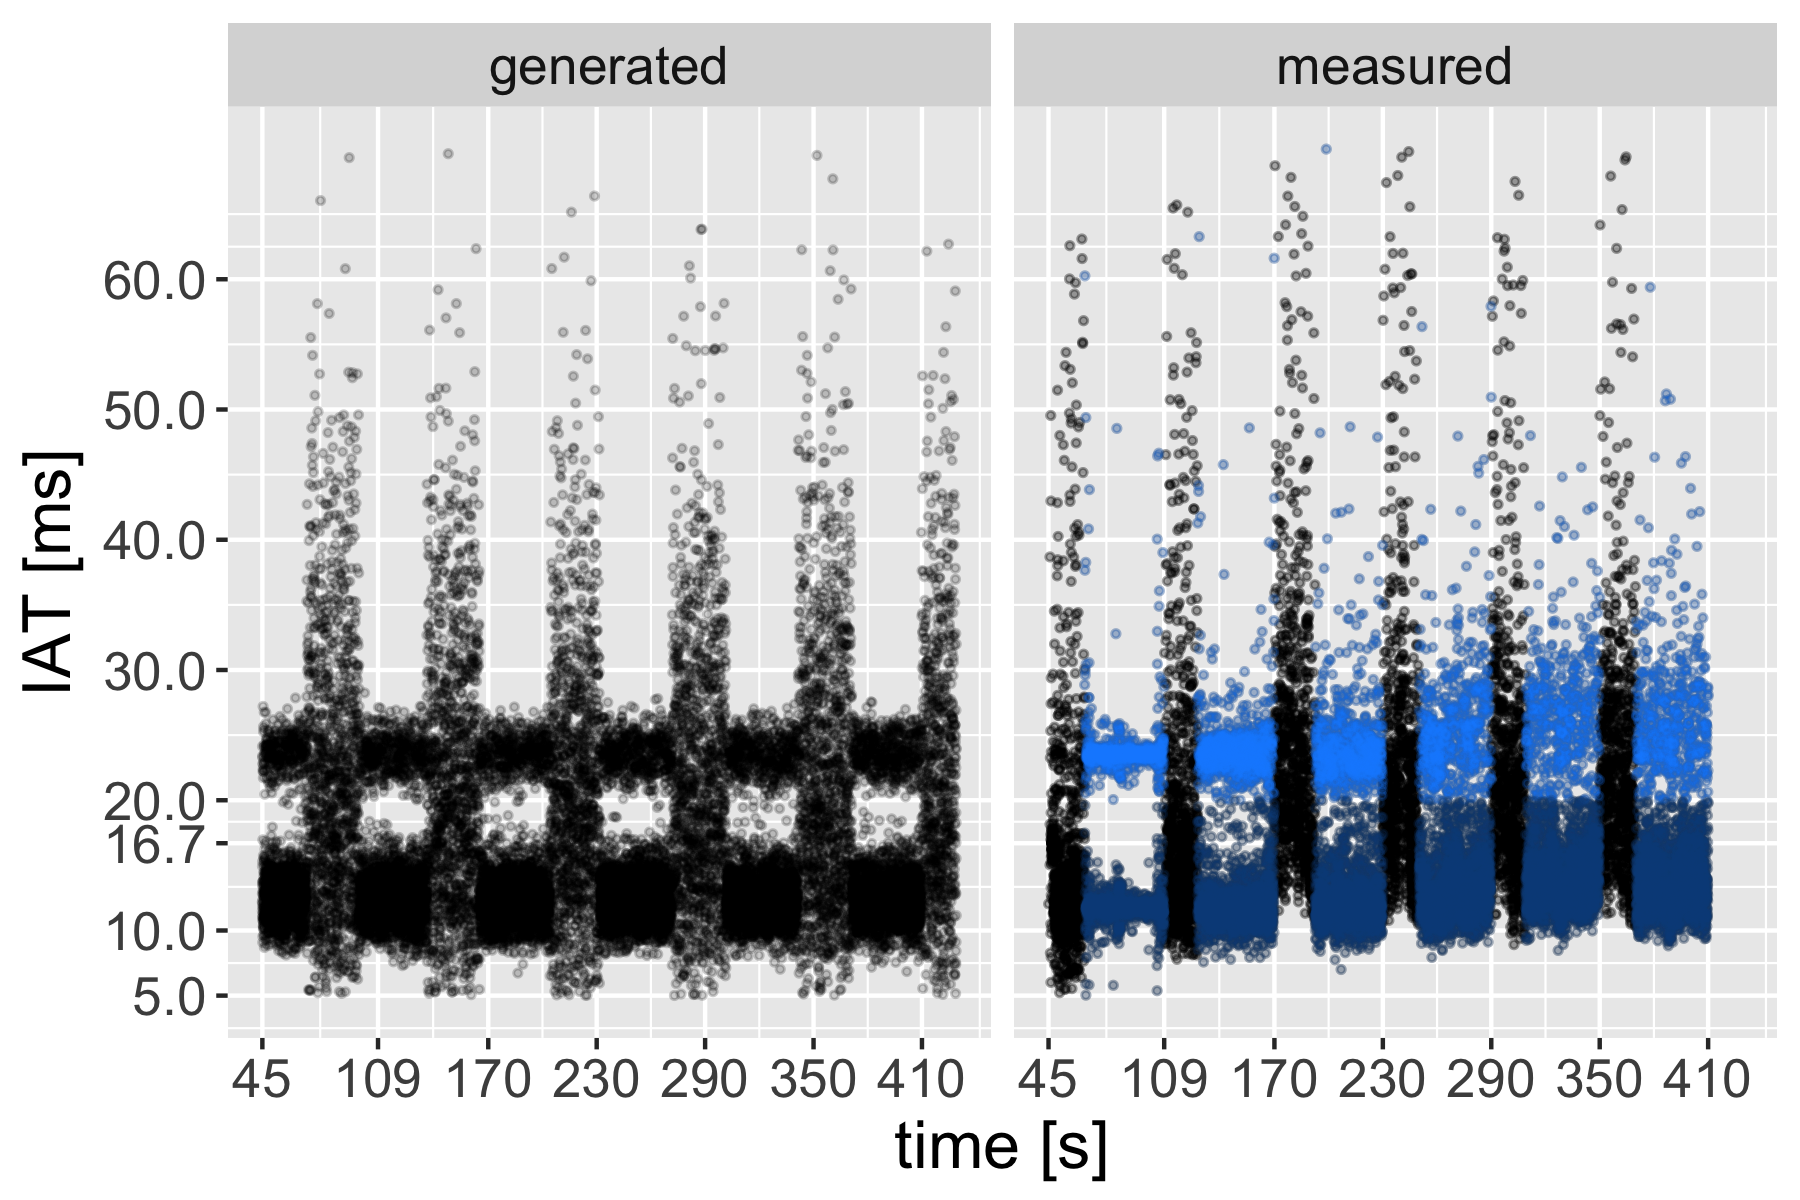
\includegraphics[width=1.0\columnwidth]{images/command-ts-annotated.png}
	\caption{Time series of the client-sent command messages both measured in the experiment as well as generated from the model. The different phases are highlighted in different colors.}
\label{fig:command-timeseries}
\end{figure}



\subsection{Game State Update Messages}

	\begin{figure}[t]
		\centering
		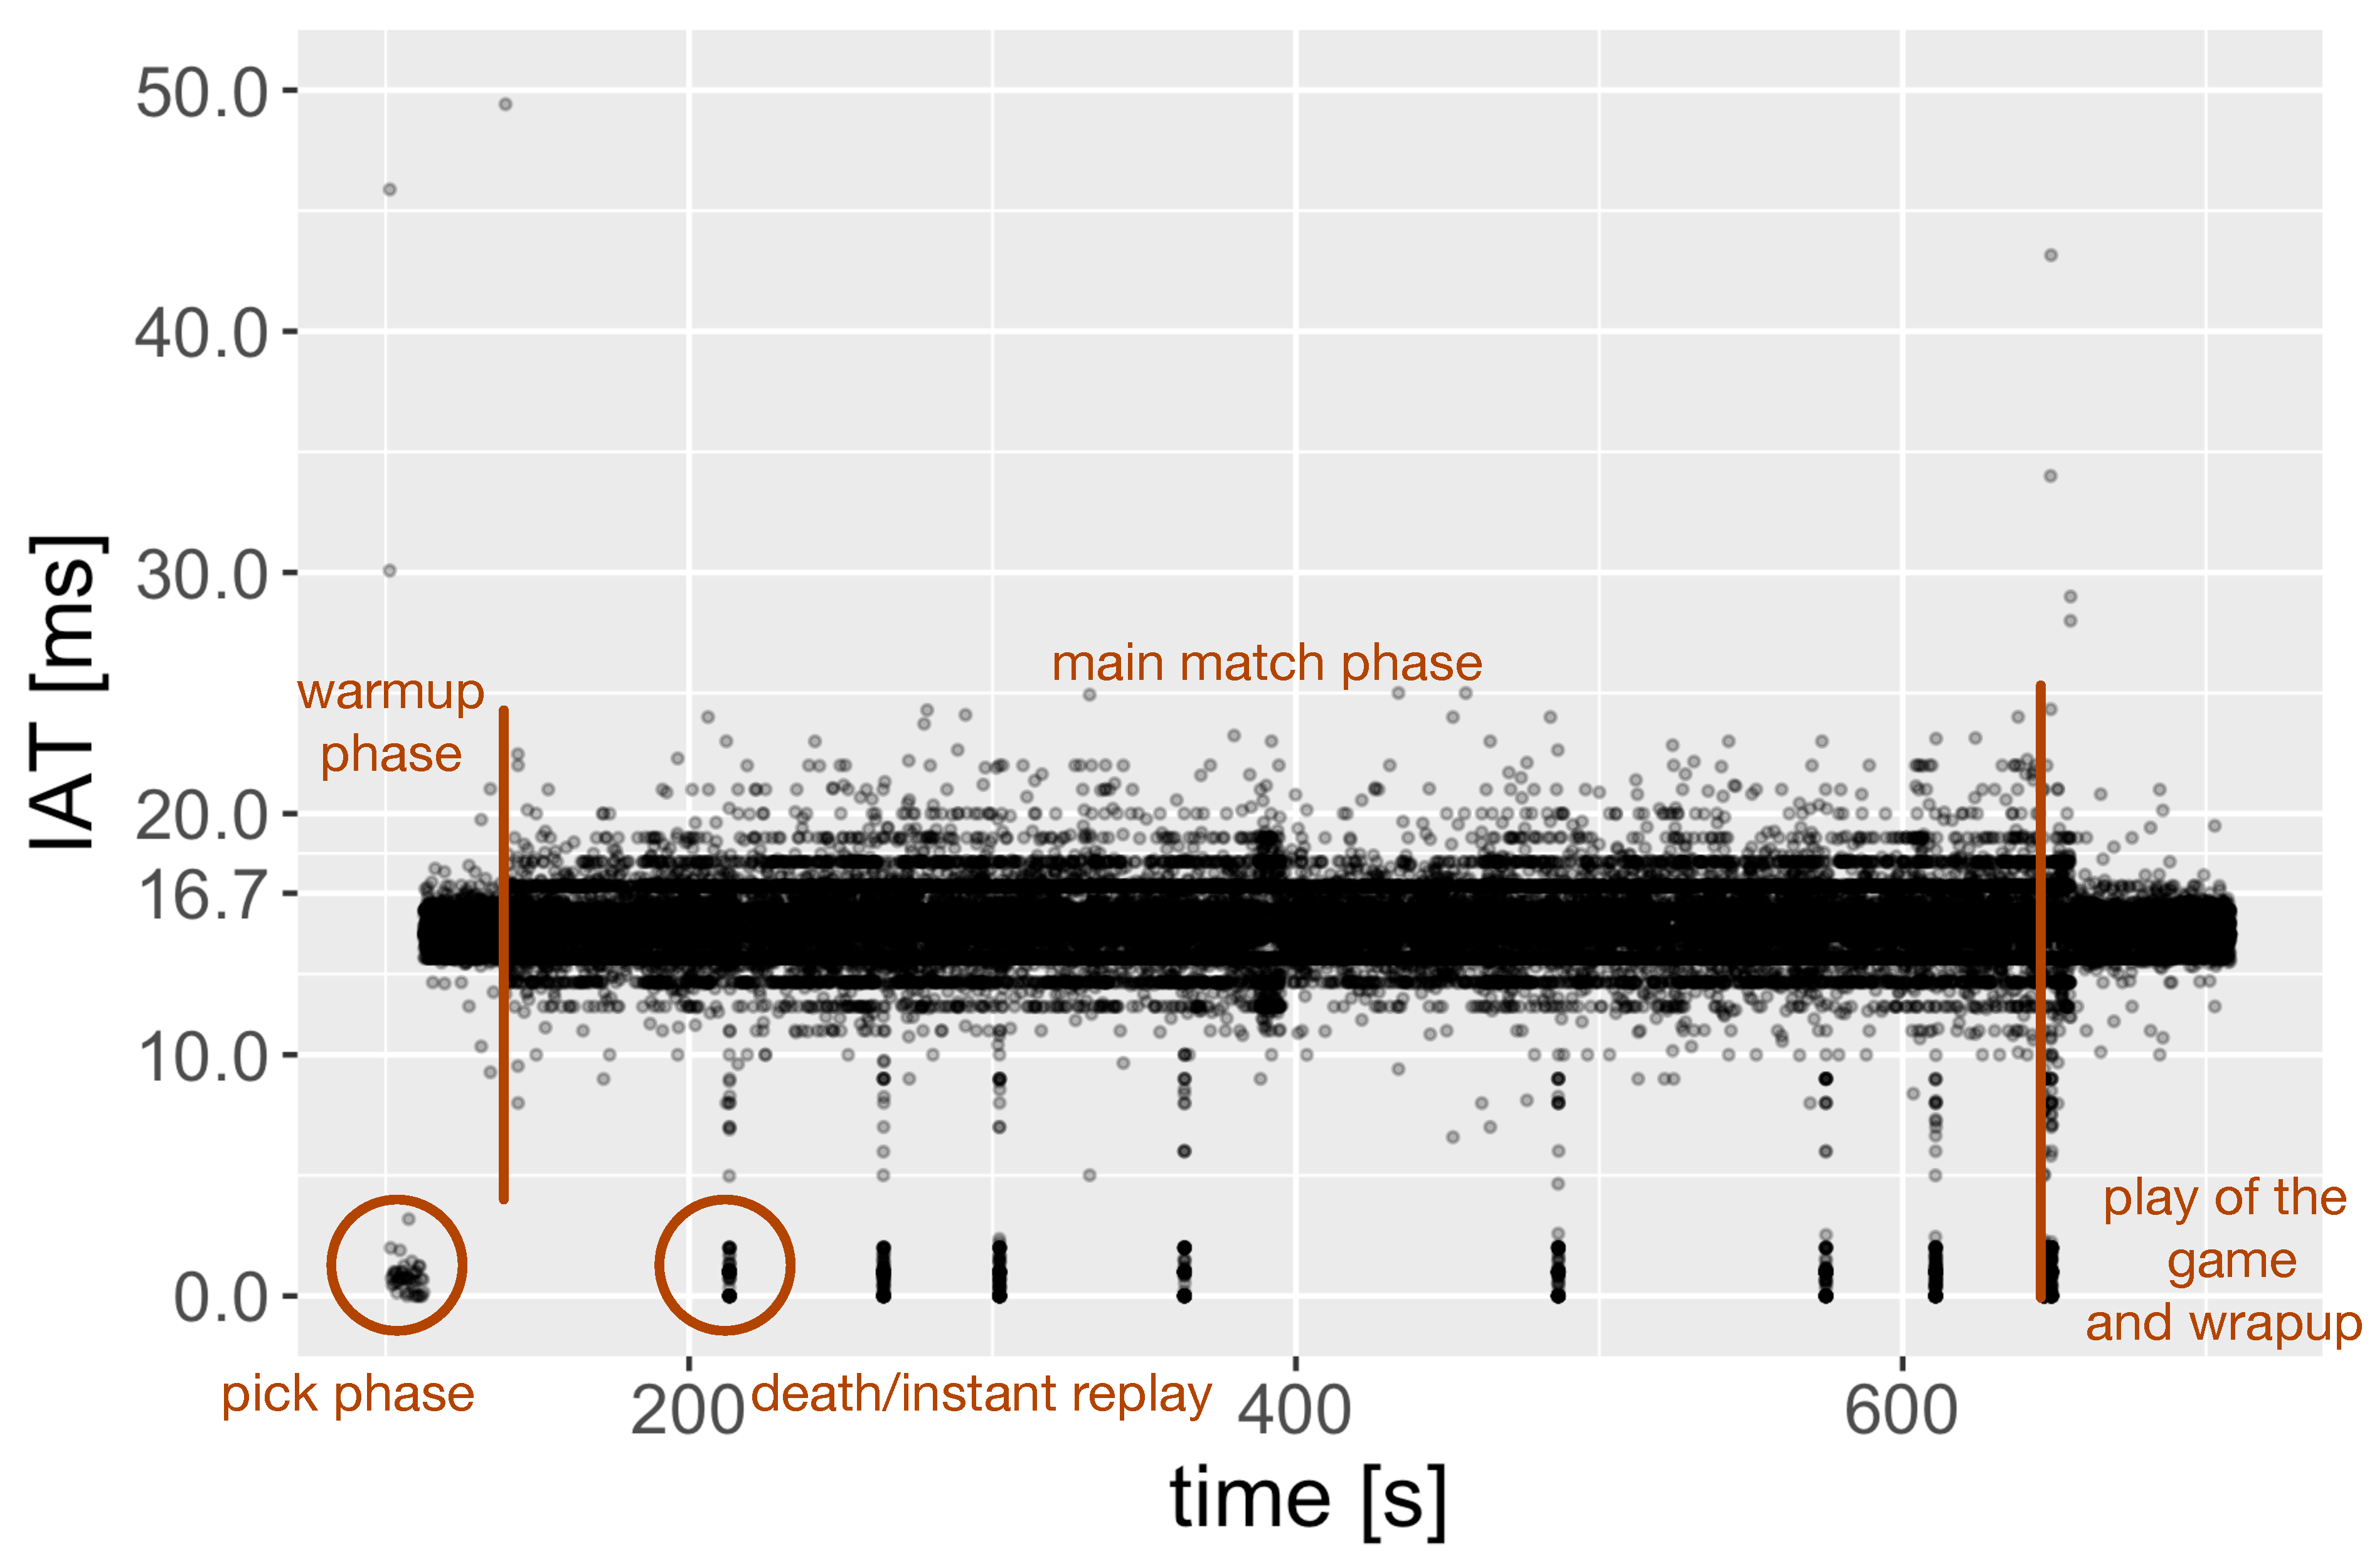
\includegraphics[width=1.0\columnwidth]{images/update-ts-annotated.pdf}
		\caption{Time series of the received game state update messages. The game phases and non-interactive ``kill cam'' events are annotated.}
	\label{fig:update-timeseries}
	\end{figure}

	\begin{figure}[t]
		\centering
		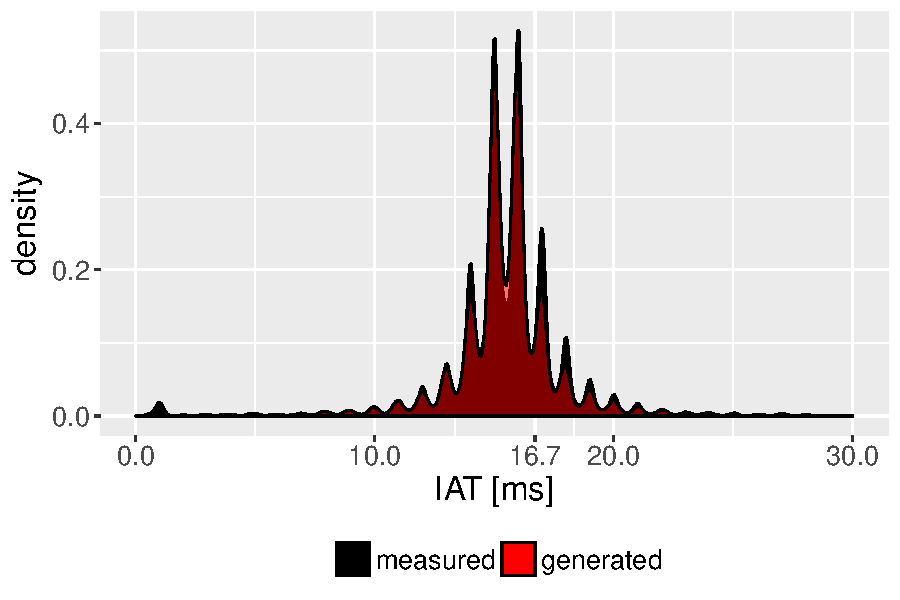
\includegraphics[width=1.0\columnwidth]{images/update-density.pdf}
		\caption{Density plot of both the measured and the fitted game state update messages received by the client.}
	\label{fig:update-density}
	\end{figure}

	The next lag component is the distribution of the game state update messages that the game server sends periodically to each connected game client. Ideally, such an update should be transmitted immediately after every game simulation ``tick''. A time series of the client's packet reception \glspl{IAT} of one match is depicted in Fig.~\ref{fig:update-timeseries}. There are a few properties of note here, that clearly indicate that the server's messaging behavior depends on the game state even though the tick rate targets a rate of \SI{60}{\hertz}. 

	The first block of very short \glspl{IAT} directly maps to the pick phase of \textsc{Overwatch}, where each player picks the hero (or class) she is going to play during this match. The next, short phase (visible by less spread in the samples) is the warmup phase, where both teams can not yet leave their respective starting areas and thus no meaningful action can occur. Only after this phase the actual game starts and the spread of the \gls{IAT} increases, possibly hinting at increased load at the server side. Similar the final phase of less sample spread depicts the game after the match has ended and the players see match statistics as well as a replay of a noteworthy event in the match (the ``Play of the Game'').

	Every now and then the data exposes a quick burst of data in short intervals (i.e. the vertical bars in Fig.~\ref{fig:update-timeseries}). This directly correlates to the so-called ``kill cam''. When the player dies during the match, and before she respawns, she is shown a quick replay of the event from the perspective of the shooter. Thus, this replay data needs to be transferred to the player first. This feature can also be turned off, eliminating the burst of data alongside.	The reason for the grouping on the vertical axis into distinctly visible horizontal bars is not entirely clear yet, but is not necessarily present on each client PC. A quick check with the game running on another computer did not exhibit this behavior. Nonetheless, it is present here and certainly influences the \gls{E2E} lag and therefore should be considered in the model.

	Due to this oscillating behavior (cf. the density plot in Fig.~\ref{fig:update-density}) the update messaging process could best be modeled with a Cauchy distribution as base, modulated with a sine function. This yields
	%
	\begin{equation*}
		f_{rcv}(x) = \frac{0.7\sin(171.6 +3120x)^4 + 0.2}{0.9848153} f(x; x_0; \gamma)^{1.17} 
	\end{equation*}
	%
	for the density, with location $x_0 = 0.0155$ and scale $\gamma = 0.0011$ for the Cauchy distribution. It should be noted that this model is only applicable for the game's main phase and excludes the ``kill cam''-events as well. Those are either not relevant to the outcome of the match (warmup phase and post-match statistics) or are even entirely non-interactive for the player.



\subsection{Input Events}

Another component is the distribution of the actual input events that the player generates with her input devices. The original simulation in \cite{Metzger+2016} just assumed an exponential distribution with a rate that might not be entirely realistic for an actual game. Therefore, for \textsc{Overwatch} the inputs were recorded and a rate parameter for the exponential distribution was derived as a compound of button strokes and mouse movements ($\lambda = 102.1824$).


\subsection{Network Delay}

Finally, the network delay must also be considered. But due to the high reliability of servers and the matchmaking that should place the player on to a server in the player's vicinity, the delay to the server should be low and stable. In a separate RTT measurement to the game server's IP address found in the investigated matches the RTT was about \SI{34}{\milli\second}. This is used as a constant network delay component in the simulation. The low variance of the measured RTT does not justify a more complex distribution here.

